\documentclass[tikz,border=3pt,convert={density=600,outext=.png}]{standalone}
%\documentclass[tikz,border=3pt]{standalone}

\usepackage[utf8]{inputenc} % utf8 encoding
\usepackage{amsmath} % nice math symbols
     

\usepackage{tikz}
\usetikzlibrary{shapes,positioning,calc,arrows,patterns}

\newcommand{\sign}[3]{
	\filldraw[fill=white] ($(0.0,0.2)+(#2,#3)$) -- ($(0.5,1.0)+(#2,#3)$) -- ($(1.0,0.2)+(#2,#3)$) -- cycle;
	\filldraw[fill=black!20] ($(0.0,0.2)+(#2,#3)$) -- ($(0.7,0.0)+(#2,#3)$) -- ($(1.0,0.2)+(#2,#3)$) -- cycle;
	
	\draw[coord_cine] ($(0.5,1.0)+(#2,#3)$) -- ($(0.5,0.13)+(#2,#3)$);
	\draw[coord_cine] ($(0.0,0.2)+(#2,#3)$) -- ($(0.5,0.13)+(#2,#3)$);
	\draw[coord_cine] ($(0.7,0.0)+(#2,#3)$) -- ($(0.5,0.13)+(#2,#3)$);
	\draw[coord_cine] ($(1.0,0.2)+(#2,#3)$) -- ($(0.5,0.13)+(#2,#3)$);
	
	\filldraw[fill=white,fill opacity=0.8] ($(0.0,0.2)+(#2,#3)$) -- ($(0.5,1.0)+(#2,#3)$) -- ($(0.7,0.0)+(#2,#3)$) -- cycle;
	\filldraw[fill=white,fill opacity=0.8] ($(0.7,0.0)+(#2,#3)$) -- ($(0.5,1.0)+(#2,#3)$) -- ($(1.0,0.2)+(#2,#3)$) -- cycle;
	
	\node[sign_comp, fill=red] (s#1_p) at ($(0.0,0.2)+(#2,#3)$) {};
	\node[sign_comp, fill=blue] (s#1_m) at ($(1.0,0.2)+(#2,#3)$) {};
	\node[sign_comp, fill=gray] (s#1_n) at ($(0.5,1.0)+(#2,#3)$) {};
	\node[sign_comp, fill=green!70!black] (s#1_a) at ($(0.7,0.0)+(#2,#3)$) {};
	
	\node[left = of s#1_p] {$p_#1$};
	\node[right = of s#1_m] {$m_#1$};
	\node[right = of s#1_n] {$n_#1$};
	\node[right = of s#1_a] {$a_#1$};
	
	\node[label] at ($(s#1_n)!0.5!(s#1_a)$) {$s_#1$};	
}
% TikZ styles for drawing

\begin{document}
	
	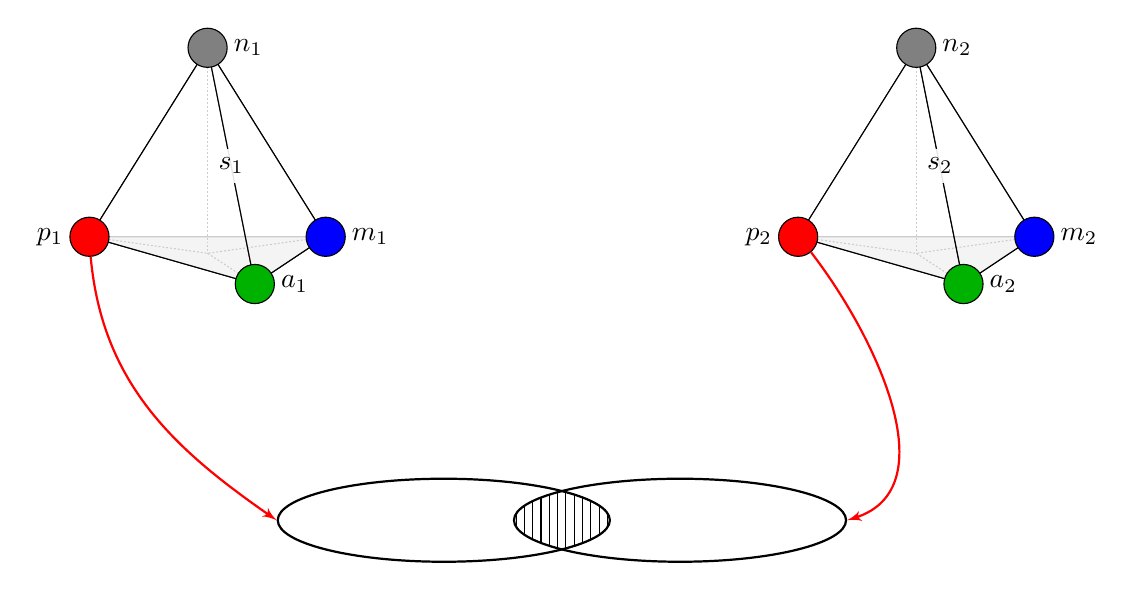
\begin{tikzpicture}[join=round,scale=3.0,node distance = -0.05]
		\tikzstyle{sign_comp}=[draw, circle, scale=1.5];
		\tikzstyle{label}=[align=center,fill=white,opacity=0.9,text opacity=1];
		\tikzstyle{coord_cine}=[dash pattern=on 0.7 off 0.7];
		
		\sign{1}{0}{0}
		\sign{2}{3}{0}
		
		\node[draw, thick, ellipse, minimum width=120, minimum height = 30] (el_1) at (1.5,-1){};
		\node[draw, thick, ellipse, minimum width=120, minimum height = 30] (el_2) at (2.5,-1){};
		\path[-latex',thick, color = red] (s1_p) edge [bend left, out = -30, in = 200] (el_1.west);
		\path[-latex',thick, color = red] (s2_p) edge [bend left, out = 30, in = 100] (el_2.east);
		
		\begin{scope}
			\clip (2.5,-1) ellipse (20pt and 5pt);
			\draw[pattern=vertical lines] (1.5,-1) ellipse (20pt and 5pt);
		\end{scope}
	\end{tikzpicture}

	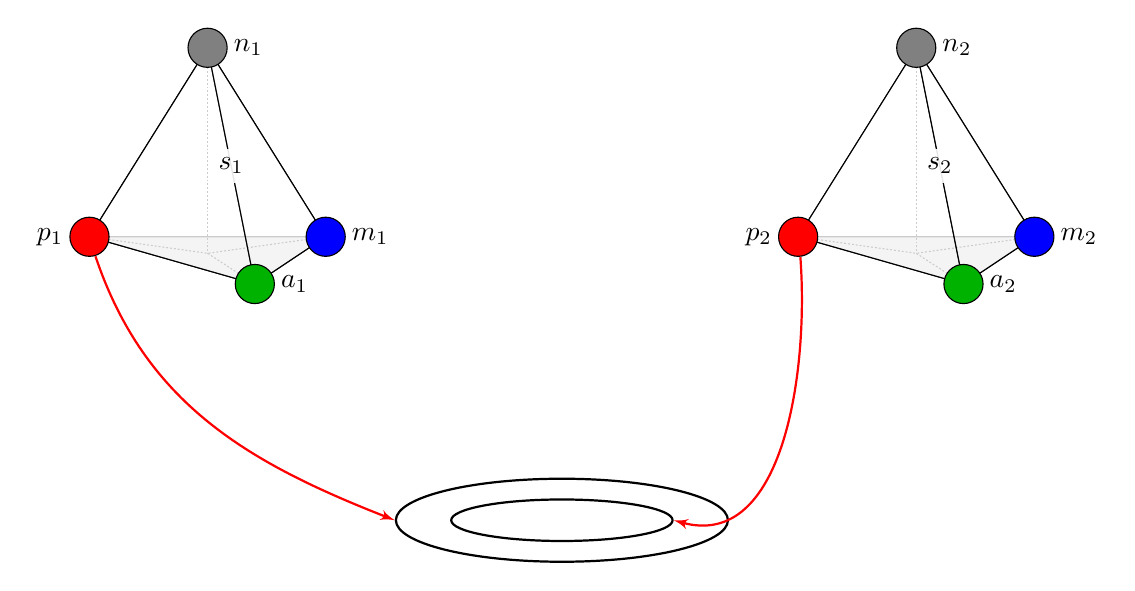
\begin{tikzpicture}[join=round,scale=3.0,node distance = -0.05]
		\tikzstyle{sign_comp}=[draw, circle, scale=1.5];
		\tikzstyle{label}=[align=center,fill=white,opacity=0.9,text opacity=1];
		\tikzstyle{coord_cine}=[dash pattern=on 0.7 off 0.7];
		
		\sign{1}{0}{0}
		\sign{2}{3}{0}
		
		\node[draw, thick, ellipse, minimum width=120, minimum height = 30] (el_1) at (2,-1){};
		\node[draw, thick, ellipse, minimum width=80, minimum height = 15] (el_2) at (2,-1){};
		\path[-latex',thick, color = red] (s1_p) edge [bend left, out = -30, in = 200] (el_1.west);
		\path[-latex',thick, color = red] (s2_p) edge [bend left, out = 30, in = 100] (el_2.east);
		
	\end{tikzpicture}
	
	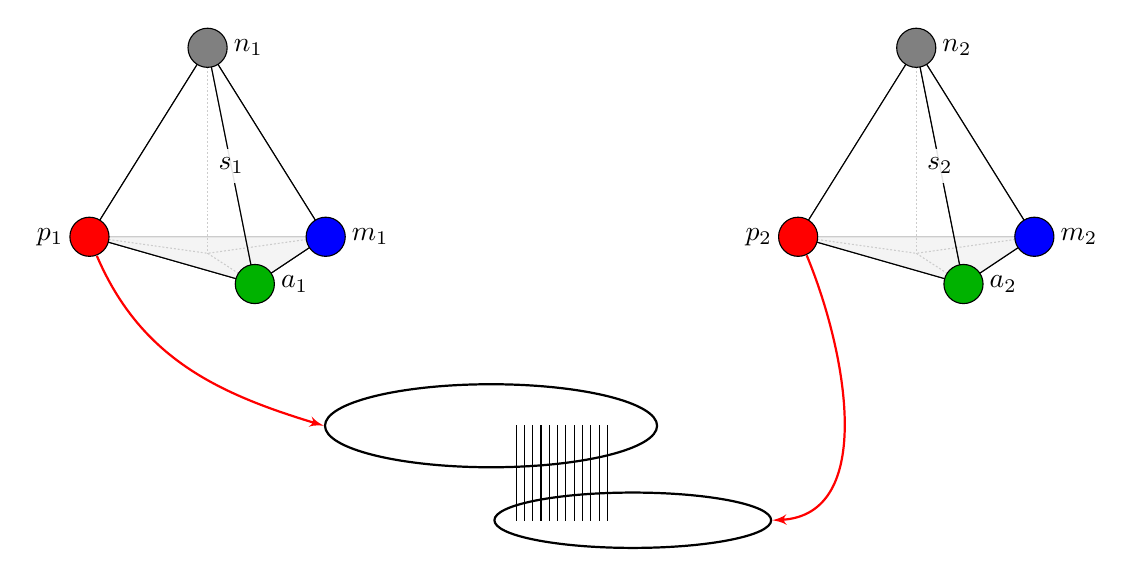
\begin{tikzpicture}[join=round,scale=3.0,node distance = -0.05]
		\tikzstyle{sign_comp}=[draw, circle, scale=1.5];
		\tikzstyle{label}=[align=center,fill=white,opacity=0.9,text opacity=1];
		\tikzstyle{coord_cine}=[dash pattern=on 0.7 off 0.7];
		
		\sign{1}{0}{0}
		\sign{2}{3}{0}
		
		\node[draw, thick, ellipse, minimum width=120, minimum height = 30] (el_1) at (1.7,-0.6){};
		\node[draw, thick, ellipse, minimum width=100, minimum height = 20] (el_2) at (2.3,-1){};
		\path[-latex',thick, color = red] (s1_p) edge [bend left, out = -30, in = 200] (el_1.west);
		\path[-latex',thick, color = red] (s2_p) edge [bend left, out = 30, in = 100] (el_2.east);
		
		\path[pattern=vertical lines] (1.8,-0.6) rectangle (2.2, -1);
	\end{tikzpicture}	
	
	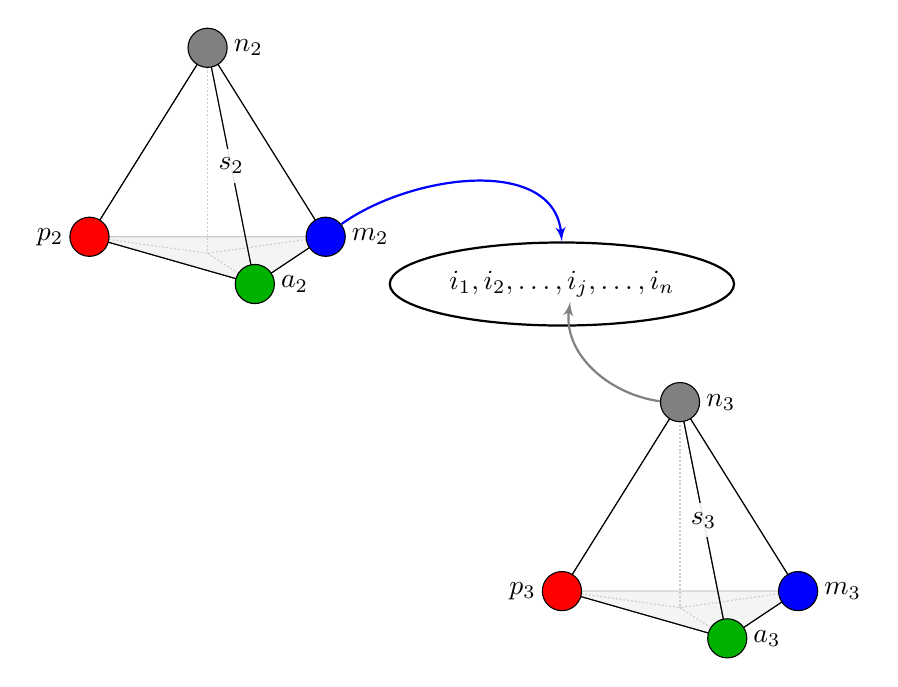
\begin{tikzpicture}[join=round,scale=3.0,node distance = -0.05]
		\tikzstyle{sign_comp}=[draw, circle, scale=1.5];
		\tikzstyle{label}=[align=center,fill=white,opacity=0.9,text opacity=1];
		\tikzstyle{coord_cine}=[dash pattern=on 0.7 off 0.7];
		
		\sign{2}{0}{1.5}
		\sign{3}{2}{0}
		
		\node[draw, thick, ellipse, minimum width=120, minimum height=30] (el_1) at (2,1.5){$i_1,i_2,\dots, i_j,\dots, i_n$};

		\path[-latex',thick, color = blue] (s2_m) edge [bend left, out = 40, in = 100] (el_1.north);
		\path[-latex',thick, color = gray] (s3_n) edge [bend left, out = 40, in = 130] ([yshift=3,xshift=1]el_1.south);
	\end{tikzpicture}
	
	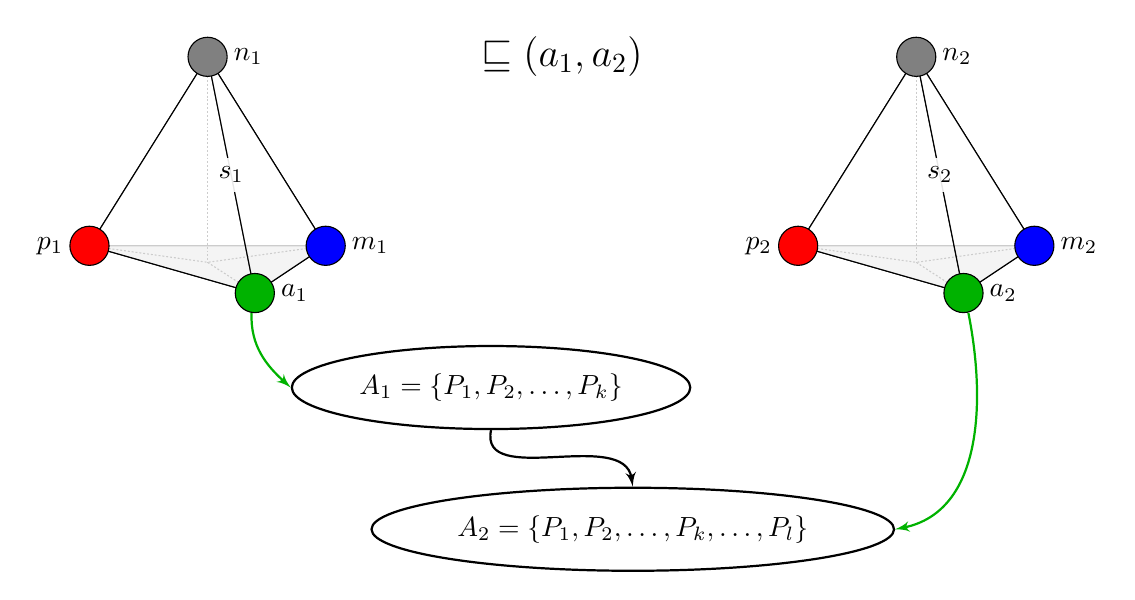
\begin{tikzpicture}[join=round,scale=3.0,node distance = -0.05]
		\tikzstyle{sign_comp}=[draw, circle, scale=1.5];
		\tikzstyle{label}=[align=center,fill=white,opacity=0.9,text opacity=1];
		\tikzstyle{coord_cine}=[dash pattern=on 0.7 off 0.7];
		
		\sign{1}{0}{0}
		\sign{2}{3}{0}
		
		\node[font=\Large] at (2,1) {$\sqsubseteq(a_1,a_2)$};
		
		\node[draw, thick, ellipse, minimum width=140, minimum height = 30] (el_1) at (1.7,-0.4){$A_1=\{P_1,P_2,\dots, P_k\}$};
		\node[draw, thick, ellipse, minimum width=140, minimum height = 30] (el_2) at (2.3,-1){$A_2=\{P_1,P_2,\dots, P_k,\dots,P_l\}$};
		\path[-latex',thick, color = green!70!black] (s1_a) edge [bend left, out = -30, in = 200] (el_1.west);
		\path[-latex',thick, color = green!70!black] (s2_a) edge [bend left, out = 30, in = 120] (el_2.east);
		\path[-latex',thick] (el_1.south) edge [bend left, out = -80, in = 120] (el_2.north);
		
	\end{tikzpicture}
	
	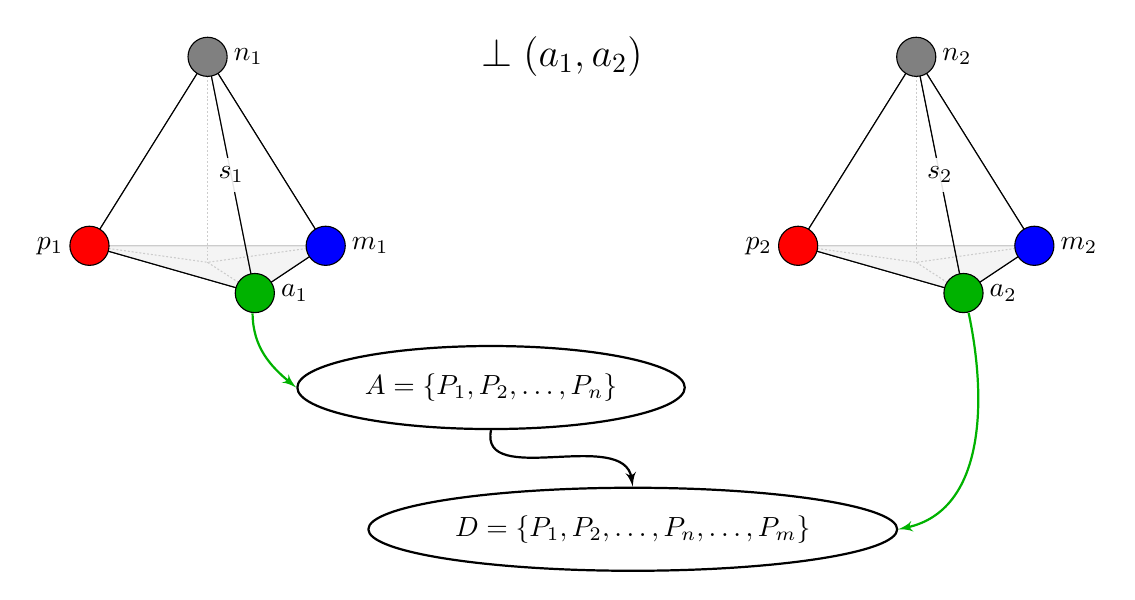
\begin{tikzpicture}[join=round,scale=3.0,node distance = -0.05]
		\tikzstyle{sign_comp}=[draw, circle, scale=1.5];
		\tikzstyle{label}=[align=center,fill=white,opacity=0.9,text opacity=1];
		\tikzstyle{coord_cine}=[dash pattern=on 0.7 off 0.7];
		
		\sign{1}{0}{0}
		\sign{2}{3}{0}
		
		\node[font=\Large] at (2,1) {$\perp(a_1,a_2)$};
		
		\node[draw, thick, ellipse, minimum width=140, minimum height = 30] (el_1) at (1.7,-0.4){$A=\{P_1,P_2,\dots, P_n\}$};
		\node[draw, thick, ellipse, minimum width=140, minimum height = 30] (el_2) at (2.3,-1){$D=\{P_1,P_2,\dots, P_n,\dots,P_m\}$};
		\path[-latex',thick, color = green!70!black] (s1_a) edge [bend left, out = -30, in = 200] (el_1.west);
		\path[-latex',thick, color = green!70!black] (s2_a) edge [bend left, out = 30, in = 120] (el_2.east);
		\path[-latex',thick] (el_1.south) edge [bend left, out = -80, in = 120] (el_2.north);
	
	\end{tikzpicture}	
	
	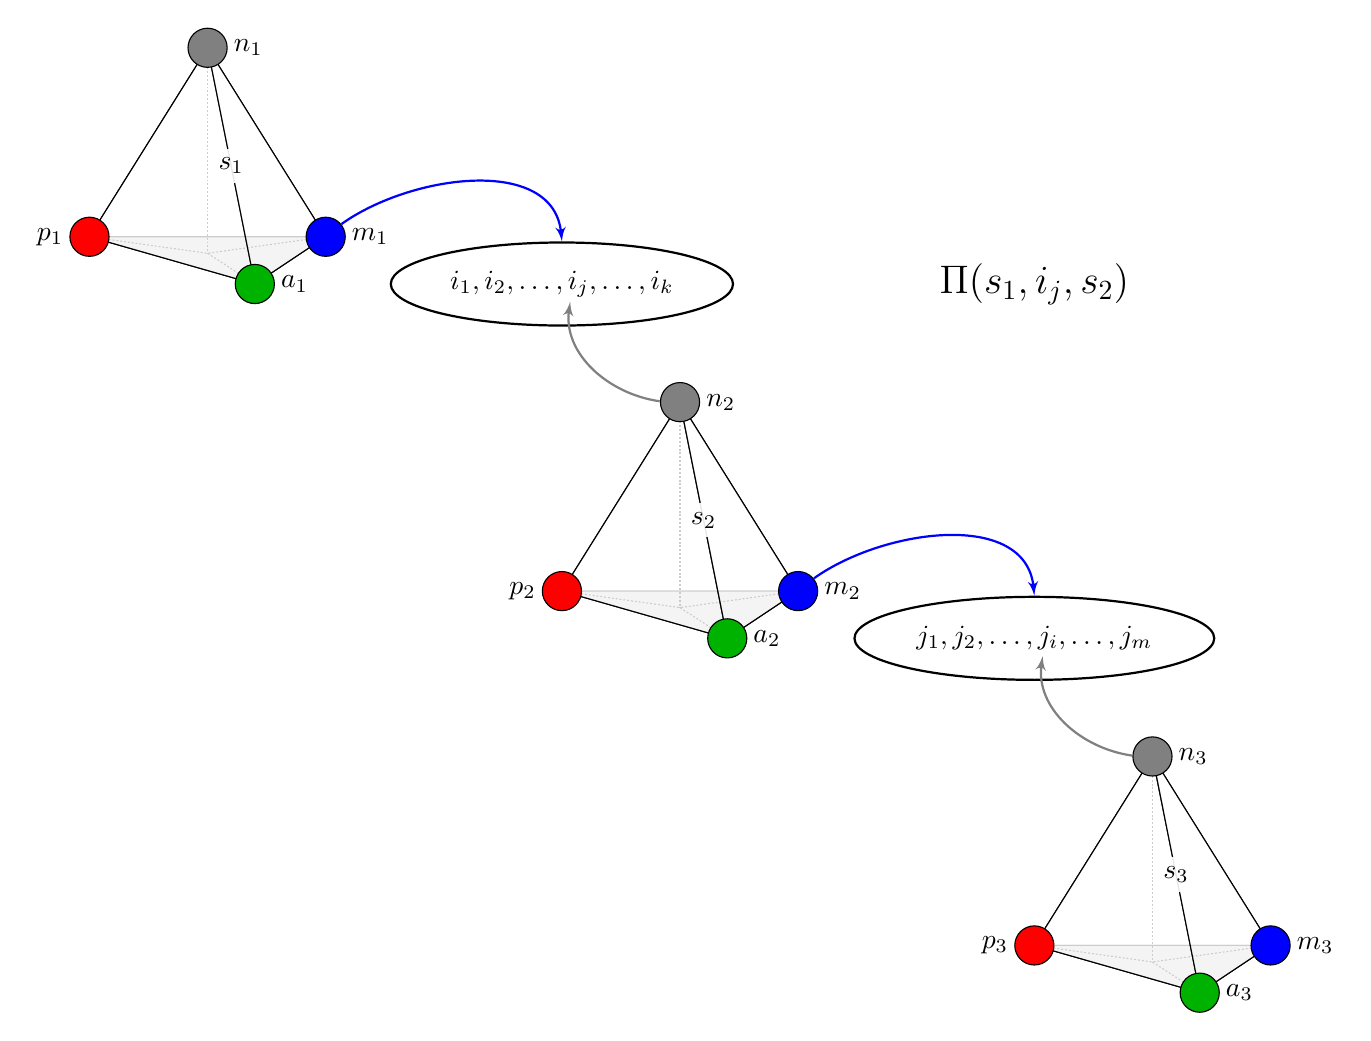
\begin{tikzpicture}[join=round,scale=3.0,node distance = -0.05]
		\tikzstyle{sign_comp}=[draw, circle, scale=1.5];
		\tikzstyle{label}=[align=center,fill=white,opacity=0.9,text opacity=1];
		\tikzstyle{coord_cine}=[dash pattern=on 0.7 off 0.7];
		
		\sign{1}{0}{1.5}
		\sign{2}{2}{0}
		\sign{3}{4}{-1.5}		
				
		\node[font=\Large] at (4,1.5) {$\Pi(s_1,i_j,s_2)$};
		
		\node[draw, thick, ellipse, minimum width=120, minimum height=30] (el_1) at (2,1.5){$i_1,i_2,\dots,i_j,\dots, i_k$};
		\node[draw, thick, ellipse, minimum width=120, minimum height=30] (el_2) at (4,0){$j_1,j_2,\dots,j_i,\dots, j_m$};
				
		\path[-latex',thick, color = blue] (s1_m) edge [bend left, out = 40, in = 100] (el_1.north);
		\path[-latex',thick, color = gray] (s2_n) edge [bend left, out = 40, in = 130] ([yshift=3,xshift=1]el_1.south);
		\path[-latex',thick, color = blue] (s2_m) edge [bend left, out = 40, in = 100] (el_2.north);
		\path[-latex',thick, color = gray] (s3_n) edge [bend left, out = 40, in = 130] ([yshift=3,xshift=1]el_2.south);
	\end{tikzpicture}	
	
	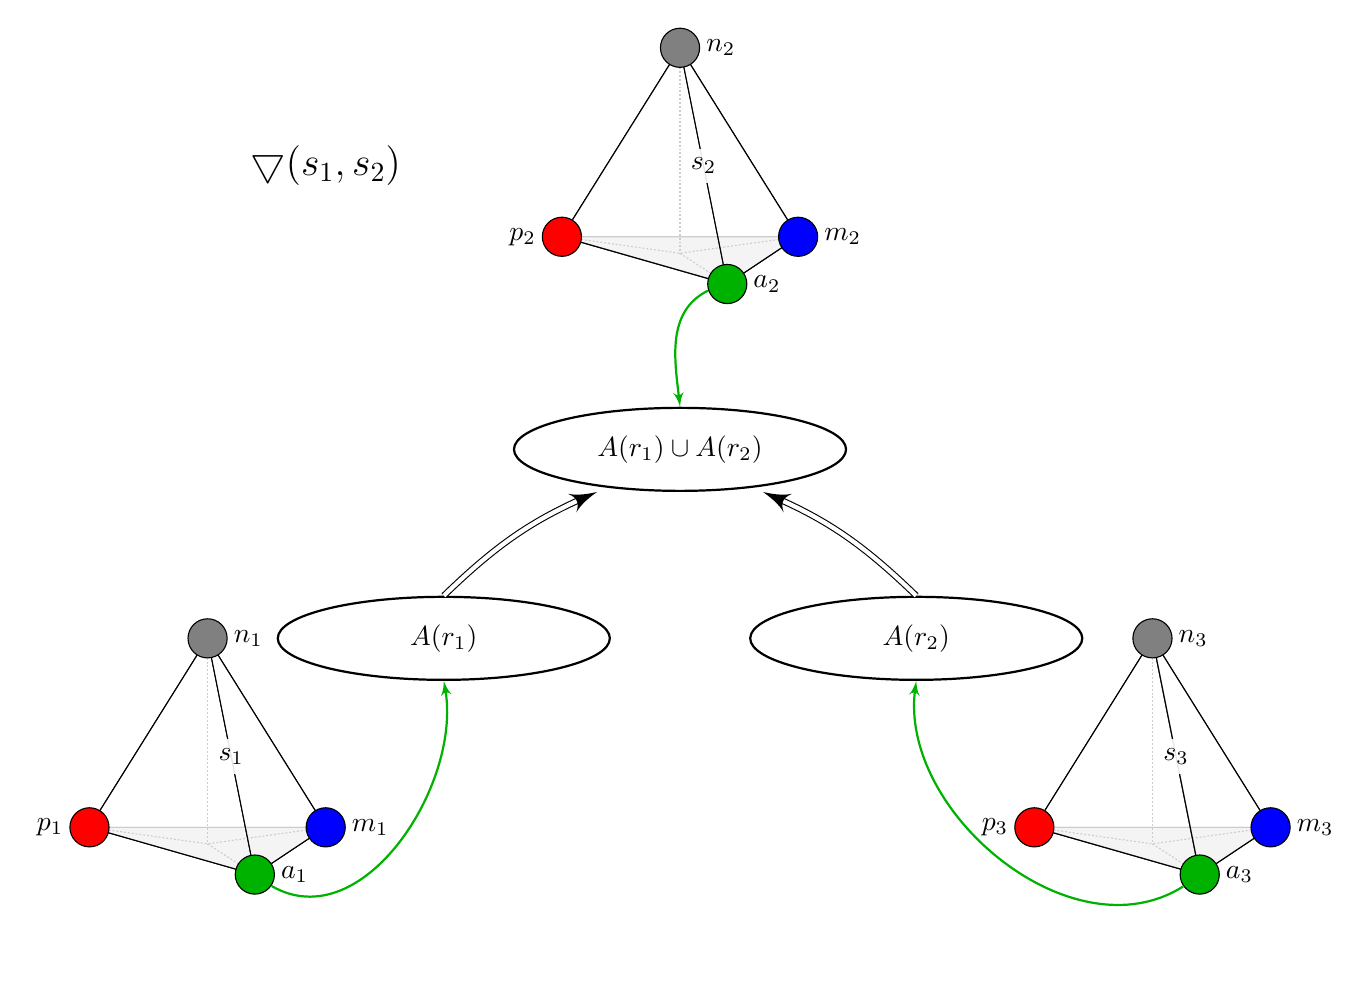
\begin{tikzpicture}[join=round,scale=3.0,node distance = -0.05]
		\tikzstyle{sign_comp}=[draw, circle, scale=1.5];
		\tikzstyle{label}=[align=center,fill=white,opacity=0.9,text opacity=1];
		\tikzstyle{coord_cine}=[dash pattern=on 0.7 off 0.7];
		
		\sign{1}{0}{0}
		\sign{2}{2}{2.5}
		\sign{3}{4}{0}
		
		\node[font=\Large] at (1,3) {$\bigtriangledown(s_1,s_2)$};
		
		\node[draw, thick, ellipse, minimum width=120, minimum height=30] (el_1) at (1.5,1){$A(r_1)$};
		\node[draw, thick, ellipse, minimum width=120, minimum height=30] (el_2) at (3.5,1){$A(r_2)$};
		\node[draw, thick, ellipse, minimum width=120, minimum height=30] (el_3) at (2.5,1.8){$A(r_1)\cup A(r_2)$};
		\path[-latex',thick, color = green!70!black] (s1_a) edge [bend left, out = -80, in = -130] (el_1.south);
		\path[-latex',thick, color = green!70!black] (s3_a) edge [bend left, out = 70, in = 120] (el_2.south);
		\path[-latex',thick, color = green!70!black] (s2_a) edge [bend left, out = -50, in = 200] (el_3.north);		
		
		\draw[-latex',double equal sign distance] (el_1.north) to[bend right=-10] ([xshift=-10]el_3.south);
		\draw[-latex',double equal sign distance] (el_2.north) to[bend left=-10] ([xshift=10]el_3.south);
	\end{tikzpicture}	
\end{document}